
\section{Validazione}

%\subsection{Scelte progettuali}


\subsection{Strumenti automatici}
Per garantire che il sito sia correttamente visualizzato e che rimanga accessibile nel maggior numero di browser possibili si è verificata la validità di tutte le pagine tramite l'utilizzo di molteplici validator e sono stati effettuati dei test di visualizzazione su browser meno recenti.

\subsubsection{Audits}
Audits è uno strumento automatizzato \textit{open-source} per migliorare la qualità delle pagine web.
I punteggi del report effettuato rappresentano una metrica dell'accessibilità e performance del sito.
\begin{figure}[H]
	\centerline{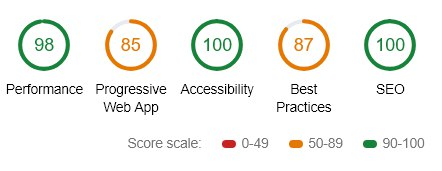
\includegraphics[scale= 0.65]{img/punteggiAudits.jpg}}
\end{figure}
Il risultato del test è stato molto buono in quanto i valori ottenuti non scendono mai sotto il punteggio di 85 su 100 massimo. 

\subsubsection{Markup Validation Service w3.org}
Tutte le pagine dell'utente generico sono state validate con questo validatore e non hanno riportato errori o warnings.

\subsubsection{W3C CSS Validator w3.org}
Tutti i fogli di stile sono stati validati con questo validatore e non hanno riportato errori.

\subsubsection{TotalValidator}
Tutte le pagine sono state validate utilizzando \textit{Total Validator}, e non hanno riportato errori.

\subsubsection{WCAG Constrast Checker}
Per la generazione di una gamma di colori accessibile, alla maggior parte dei disturbi visivi, è stato usato il validator \textit{WCAG Constrast Checker}. Il test effettuato non ha riportato errori rispetto agli standard del W3C.
\subsection{Test effettuati}

\subsubsection{Browser}
Il sito è stato testato con successo su i seguenti browser: Google Chrome, Mozilla Firefox e Internet Explorer. Nessuno di questi browser ha dato problemi riguardanti l'utilizzo e le funzionalità del sito.

\subsubsection{Mobile}
Sono stati effettuati dei test anche per la versione mobile, in particolare su i seguenti modelli:
\begin{itemize}
	\item Huawei Honor 9;
	\item Iphone 6; 
	\item Motorola G6 plus;
\end{itemize}
L’usabilità del sito web rimane invariata per ogni dispostivo essendo stato sviluppato in modo da essere responsive.

\subsubsection{Screen reader}
Tutte le pagine del sito sono stato testate dallo \textit{screen reader} per non vedenti Nvda, Non visual desktop access, e non hanno dato problemi o warnings. 

